% Marco teórico - Microfísica
%\chapter{Microfísica: Ecuaciones de Estado}
%\thispagestyle{fancy}

% Introducción similar al capítulo sobre macrofísica. Aquí queremos mostrar brevemente la motivación de el estudio de ecuaciones de estado para entender la física de la materia en entornos tan densos y de tan alta energía.

%\section{Ecuaciones de Estado y Ejemplos}

%Definir las ecuaciones de estado (en este caso barótropas) y mostrar brevemente modelos y gráficas de modelos más simples: gas degenerado de neutrones, protones y electrones libres

%\section{Teoría Relativista de Campo Medio}

% Introducir la RMFT y mostrar las ventajas de una teoría relativista efectiva de campos mesónicos que se toman como uniformes mediante su valor medio en el estado base, frente a otros métodos como QCD y los Scrhodinger-based. Hablar sobre las simetrías y sus cantidades conservadas para explicar como se obtiene la expresión para la densidad de energía y de presión en una teoría de este estilo, construida sobre un lagrangeano.

%\section{Modelo del Estudio}

% Introducir el lagrangiano para un modelo que contenga neutrones, protones, electrones (campos esponoriales); un mesón escalar neutro sigma con autointeracciones de hasta 4to orden acoplado a la densidad escalar de nucleones, un mesón vectorial neutro omega acoplado a la corriente vectorial de nucleones y un mesón vectorial isovectorial neutro rho acoplado a la corriente de isospín de nucleones. Luego hallar las ecuaciones de movimiento para los campos, para finalmente llegar a la expresión de densidad de energía y presión. Hablar sobre los parámetros libres de este modelo.

%\subsection{Materia en Saturación Nuclear}

% Definir, explicar (importancia) y mostrar las mediciones de densidad de saturación, energía de enlace por nucleón, modulo de compresión, coeficiente de energía de simetría y pendiente del coeficiente de energía de simetría. Tomar las mismas mediciones de la propuesta.

\thispagestyle{fancy}
\chapter{Microfísica: Ecuaciones de Estado}

La descripción microscópica de la materia en entornos extremos de densidad es un problema de gran complejidad en la física moderna. En estas condiciones, con densidades que exceden significativamente la densidad nuclear de saturación, la materia exhibe comportamientos que requieren marcos teóricos que incorporen efectos relativistas y de muchos cuerpos. La ecuación de estado que gobierna esta materia establece la conexión directa entre la física microscópica de las interacciones nucleares y las propiedades macroscópicas observables de las estrellas de neutrones \cite{oppenheimerMassiveNeutronCores1939}.

La teoría relativista de campo medio surge como una herramienta particularmente adecuada para abordar este régimen, brindando un tratamiento consistente que respeta la causalidad mientras incorpora las interacciones nucleares fuertes \cite{glendenningCompactStarsNuclear2000}. Este formalismo permite extrapolar desde las propiedades conocidas de materia nuclear simétrica hacia las condiciones asimétricas y de alta densidad relevantes para objetos compactos.

\section{Ecuaciones de Estado y Ejemplos}

Una ecuación de estado define la relación termodinámica entre las variables que caracterizan el estado de equilibrio de un sistema físico. Para materia estelar a temperatura cero, consideramos ecuaciones de estado barotrópicas que relacionan la presión $P$ con la densidad de energía $\rho$ mediante (\ref{eq:ecuacion_estado}). Esta relación contiene toda la información termodinámica necesaria para determinar la estructura de equilibrio hidrostático de estrellas de neutrones a través de las ecuaciones de Tolman-Oppenheimer-Volkoff (\sistemaTOV). La aproximación barotrópica es válida cuando los tiempos y escalas característicos de los procesos térmicos son despreciables comparados con las escalas hidrodinámicas y gravitacionales que determinan la estructura estelar. Se desprecia la temperatura debido a que la energía térmica y sus efectos son varios órdenes de magnitud inferiores a las energías internas de la materia en estrellas de neutrones \cite{shapiroBlackHolesWhite2008}.

\subsection{Ejemplo: Ecuación Politrópica}

La ecuación de estado politrópica es uno de los modelos más sencillos para describir materia estelar, estableciendo una relación de ley de potencias entre la presión y la densidad de masa:

\begin{equation}
	P = K \rho^{\gamma},
	\label{eq:eos_politropica}
\end{equation}

donde $K$ es una constante politrópica y $\gamma$ es el índice adiabático. Esta forma funcional, aunque fenomenológica, captura comportamientos asintóticos importantes de sistemas físicos más complejos y brinda soluciones analíticas o semi-analíticas para las ecuaciones de estructura estelar. El índice politrópico $n = 1/(\gamma - 1)$ determina las características de compresibilidad del material: valores bajos de $n$ corresponden a materia incompresible, mientras que valores altos describen sistemas altamente compresibles. Para materia ultra-relativista, $\gamma = 4/3$ ($n = 3$), mientras que para materia no-relativista degenerada, $\gamma = 5/3$ ($n = 3/2$) \cite{chandrasekharIntroductionStudyStellar1970}.

\subsection{Ejemplo: Gas Ideal Degenerado}
\label{sec:gasnpe}

Los modelos más realistas consideran gases degenerados de fermiones. Para materia nuclear compuesta por neutrones, protones y electrones, la ecuación de estado completa debe incluir las contribuciones de todas las especies presentes \cite{shapiroBlackHolesWhite2008}:

\begin{align}
	\rho_{\text{total}} &= \rho_n + \rho_p + \rho_e, \label{eq:densidad_total} \\
	P_{\text{total}} &= P_n + P_p + P_e, \label{eq:presion_total}
\end{align}

donde cada componente fermionica contribuye según:

\begin{align}
	\rho_i &= \frac{g_i}{8\pi^2} \int_0^{p_{Fi}} p^2\sqrt{p^2 + m_i^2} \, dp, \label{eq:densidad_fermi_general} \\
	P_i &= \frac{g_i}{24\pi^2} \int_0^{p_{Fi}} \frac{p^4}{\sqrt{p^2 + m_i^2}} \, dp, \label{eq:presion_fermi_general}
\end{align}

con masas $m_n = 939.6$ MeV, $m_p = 938.3$ MeV, $m_e = 0.511$ MeV y degeneraciones estadísticas (de espín) $g_i = 2$ para todas las especies. Los momentos de Fermi $p_{Fi}$ están determinados por las densidades de número mediante $n_i = \frac{g_i p_{Fi}^3}{6\pi^2}$, de modo que se tienen tres cantidades independientes: las densidades de número de las diferentes especies. Para resolver el sistema, se imponen restricciones adicionales sobre la composición de la materia garantizando el equilibrio termodinámico: la neutralidad de carga eléctrica requiere $n_p = n_e$, mientras que el equilibrio beta débil $n \rightleftharpoons p + e^- + \bar{\nu}_e$ establece la condición $\mu_n = \mu_p + \mu_e$ entre los potenciales químicos, asumiendo que los neutrinos escapan del sistema sin alterar su energía. Estas restricciones permiten expresar todas las densidades en función de un parámetro libre como el momento de Fermi del electrón $p_{Fe}$, lo que reduce el sistema a una parametrización unidimensional.

\begin{figure}[h]
	\centering
	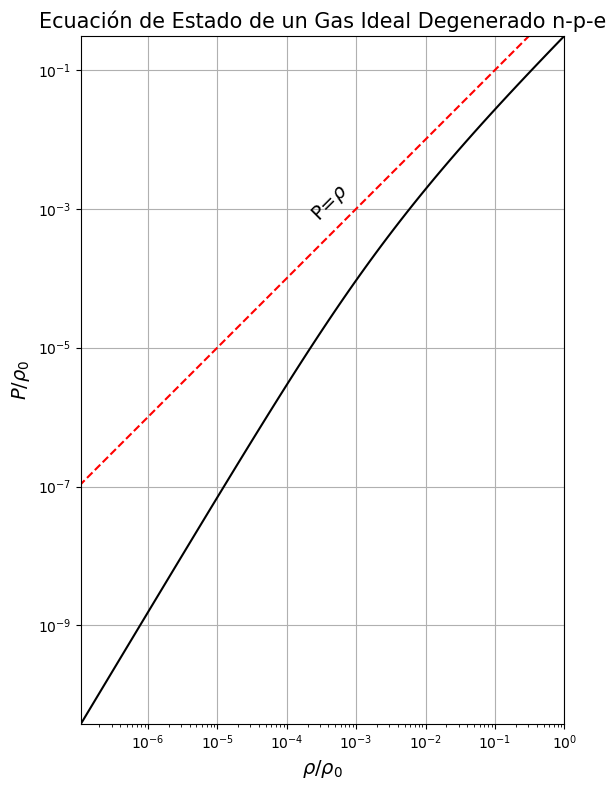
\includegraphics[width=0.55\linewidth]{Figuras/gas_npe}
	\caption{Ecuación de estado normalizada de un gas ideal degenerado de neutrones, protones y electrones. La ecuación de estado es causal ($c_s^2 = dP/d\rho < 1$).}
	\label{fig:eosnpe}
\end{figure}

Las integrales (\ref{eq:densidad_fermi_general}) y (\ref{eq:presion_fermi_general}) son analíticas, de modo que la ecuación de estado queda determinada por las expresiones $\rho(n_e)$ y $P(n_e)$ interpoladas sobre un rango de densidades relevante para estrellas de neutrones. El resultado de esta ecuación de estado se muestra en la figura \ref{fig:eosnpe}. Luego, empleando las ecuaciones TOV (\sistemaTOV) obtenemos las masas y radios de estrellas construidas con este material, como se muestra en la figura \ref{fig:mrnpe}. Este modelo sencillo predice una masa máxima de apenas 0.7$\masasol$, muy inferior a las masas que se han observado recientemente de estrellas de neutrones, listadas en la sección \ref{sec:obsNS}.

\begin{figure}
	\centering
	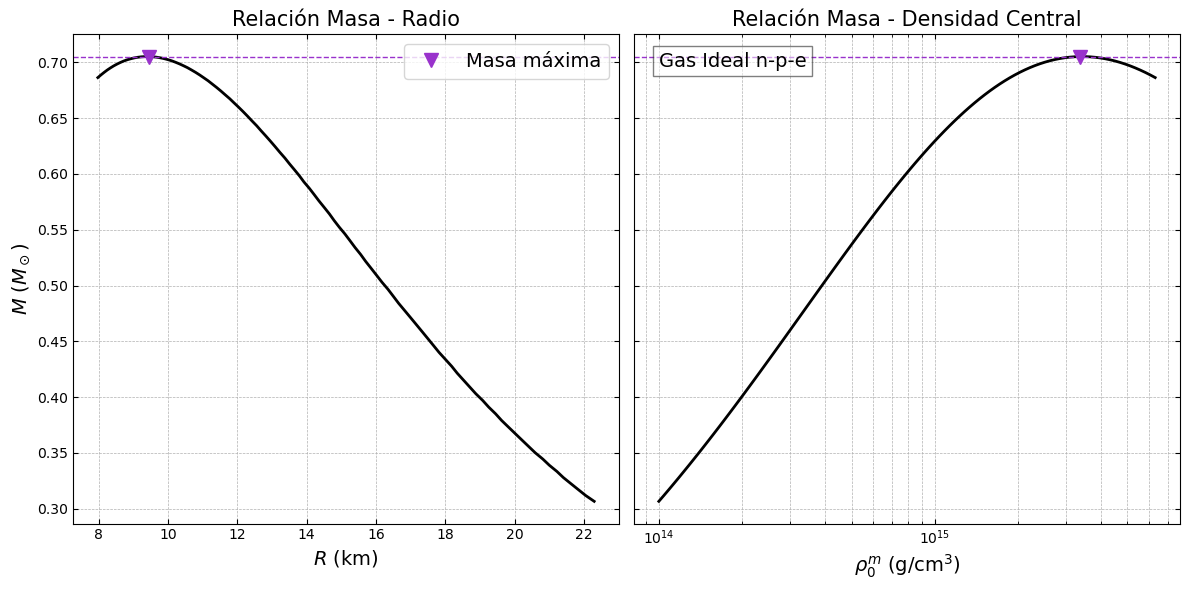
\includegraphics[width=0.9\linewidth]{Figuras/gas_npe_MR}
	\caption{Relaciones de masa - radio y masa - densidad central de masa de estrellas de neutrones constituidas por un gas ideal de neutrones, protones y electrones libres.}
	\label{fig:mrnpe}
\end{figure}



\section{Teoría Relativista de Campo Medio}

La teoría relativista de campo medio es un marco teórico que describe las interacciones nucleares mediante el intercambio de mesones efectivos, extendiendo el modelo de gas degenerado (discutido en \ref{sec:gasnpe}) e incorporando naturalmente las características relativistas en condiciones de alta densidad. Formulada por Walecka en 1974 \cite{waleckaTheoryHighlyCondensed1974}, esta aproximación ofrece ventajas significativas respecto a enfoques no-relativistas basados en potenciales fenomenológicos, particularmente en su construcción covariante, su capacidad para reproducir simultáneamente las propiedades de saturación nuclear, el comportamiento asintótico a alta densidad, y la consistencia causal relativista. Adicionalmente, al ser una teoría efectiva, requiere de un menor esfuerzo computacional respecto a teorías más fundamentales como QCD.

El formalismo se construye a partir de un lagrangiano que describe nucleones interactuando a través de campos mesónicos. Los campos fermiónicos representan los grados de libertad nucleónicos y leptónicos, mientras que los campos bosónicos representan mesones que median las interacciones fuertes. La aproximación de campo medio consiste en reemplazar los operadores de campo mesónicos por sus valores esperados en el estado base degenerado:

\begin{equation}
	\langle \phi_i(x^\mu) \rangle = \phi_i^0 \equiv \text{constante},
	\label{eq:campo_medio}
\end{equation}

donde $\phi_i$ denota los diferentes campos mesónicos del modelo. Esta aproximación es válida cuando las fluctuaciones cuánticas son pequeñas comparadas con los valores esperados de los campos, condición que se satisface en materia nuclear densa cuanto mayor es la densidad del sistema \cite{waleckaRelativisticNuclearManyBody1986}.

\subsection{Simetrías y Conservaciones}

El formalismo de la teoría se construye sobre la teoría cuántica de campos. La densidad lagrangiana $\mathcal{L}(\psi, \partial_\mu \psi, \phi_a, \partial_\mu \phi_a)$ describe las interacciones entre campos fermiónicos $\psi$ y campos bosónicos $\phi_a$ junto con sus términos libres. Esta densidad lagrangiana debe satisfacer los requerimientos de localidad, covariancia de Lorentz, y las simetrías internas relevantes para las interacciones nucleares fuertes \cite{glendenningCompactStarsNuclear2000}. La acción del sistema se define como la integral de la densidad lagrangiana sobre el volumen espaciotemporal:

\begin{equation}
	S[\psi, \phi_a] = \int d^4x \, \mathcal{L}(\psi, \partial_\mu \psi, \phi_a, \partial_\mu \phi_a),
	\label{eq:accion}
\end{equation}

donde $d^4x$ es el elemento de volumen en coordenadas de Minkowski. El principio de acción estacionaria establece que las configuraciones físicas de los campos corresponden a los extremos de esta funcional, lo que conduce a las ecuaciones de movimiento mediante el cálculo variacional. Las ecuaciones de Euler-Lagrange para todos los campos son:

\begin{equation}
	\frac{\partial \mathcal{L}}{\partial \varphi_b} - \partial_\mu \left( \frac{\partial \mathcal{L}}{\partial (\partial_\mu \varphi_b)} \right) = 0,
	\label{eq:euler_lagrange}
\end{equation}

donde $\varphi_b$ representa todos los campos presentes. Estas ecuaciones se calculan para cada componente de los campos antes de aplicar la aproximación de campo medio, obteniendo el sistema de ecuaciones de movimiento a resolver. La teoría presenta simetrías externas e internas que determinan sus conservaciones y sus consecuencias físicas. Las simetrías externas son las transformaciones del grupo de Poincaré: traslaciones espaciotemporales $x^\mu \mapsto x'^\mu = x^\mu + a^\mu$ y boosts de Lorentz $x^\mu \mapsto x'^\mu = \Lambda^\mu{}_\nu x^\nu$. Las simetrías internas relevantes incluyen la simetría de gauge global $U(1)$ $\psi \mapsto e^{-i\lambda}\psi$ asociada con la conservación del número bariónico, y la simetría de isospín $SU(2)$ $\psi \mapsto e^{-i\boldsymbol{\tau}\cdot\boldsymbol{\lambda}}\psi$ asociada con la relación entre neutrones y protones, en la aproximación de iguales masas.

El teorema de Noether establece una correspondencia entre simetrías continuas del lagrangiano y cantidades conservadas. Para cada simetría continua existe una corriente conservada correspondiente que satisface una ecuación de continuidad. El tensor de energía-momento, asociado a la simetría externa, se define como:

\begin{equation}
	T^{\mu\nu} = \frac{\partial \mathcal{L}}{\partial (\partial_\mu \varphi_j)} \partial^\nu \varphi_j - \eta^{\mu\nu} \mathcal{L}, \quad \partial_\mu T^{\mu\nu} = 0,
	\label{eq:tensor_energia_momento}
\end{equation}

garantizando que la energía total ($T^{00}$) y el momento total ($T^{0i}$) del sistema se conserven en el tiempo en ausencia de fuerzas externas.

La corriente bariónica, asociada a la simetría interna $U(1)$, se define como:

\begin{equation}
	J_B^\mu = \sum_N \bar{\psi}_N \gamma^\mu \psi_N, \quad \partial_\mu J_B^\mu = 0,
	\label{eq:corriente_barionica}
\end{equation}

donde la suma se extiende sobre todas las especies de bariones presentes. Esto implica que el número bariónico total $\int d^3x \, J_B^0$ integrado sobre el volumen total del sistema considerado, permanece constante en el tiempo reflejando el hecho experimental de que los bariones no se crean ni se destruyen en interacciones fuertes.

La corriente de isospín, asociada a la simetría interna $SU(2)$, se define como:

\begin{equation}
	\boldsymbol{J}_I^{\mu} = \sum_N \bar{\psi}_N \gamma^\mu \frac{\boldsymbol{\tau}}{2} \psi_N, \quad \partial_\mu J_I^{\mu a} = 0,
	\label{eq:corriente_isospin}
\end{equation}

donde $\boldsymbol{\tau} = \tau^a$ ($a = 1, 2, 3$) son las matrices de Pauli en el espacio de isospín. Aunque en la realidad física esta simetría está ligeramente rota por las diferencias de masa entre neutrones y protones y por las interacciones electromagnéticas, en la aproximación de igual masa se cumple. La conservación aproximada de isospín justifica el tratamiento unificado de neutrones y protones en modelos de materia nuclear simétrica.

Estas leyes de conservación derivadas del teorema de Noether añaden restricciones importantes sobre la dinámica del sistema y establecen conexiones directas entre las simetrías fundamentales de la teoría y las cantidades físicamente observables.


\section{Modelo del Estudio}

%El modelo específico empleado en este trabajo se basa en un lagrangiano relativista que incorpora nucleones y leptones interactuando mediante campos mesónicos escalares e isovectoriales. El lagrangiano total incluye términos para nucleones (campos espinoriales), un mesón escalar neutro $\sigma$ con autointeracciones no-lineales hasta cuarto orden, un mesón vectorial neutro $\omega$, y un mesón vectorial isovectorial $\rho$ \cite{glendenningCompactStarsNuclear2000}:
%
%\begin{align}
%	\mathcal{L} = &\sum_{N=n,p} \bar{\psi}_N \left[ \gamma^\mu \left( i\partial_\mu - g_{\omega N} \omega_\mu - g_{\rho N} \boldsymbol{\tau}_N \cdot \boldsymbol{\rho}_\mu \right) - (m_N - g_{\sigma N} \sigma) \right] \psi_N \nonumber \\
%	&+ \frac{1}{2} \left( \partial_\mu \sigma \partial^\mu \sigma - m_\sigma^2 \sigma^2 \right) - \frac{g_2}{2} \sigma^3 - \frac{g_3}{6} \sigma^4 \nonumber \\
%	&- \frac{1}{4} \omega_{\mu\nu} \omega^{\mu\nu} + \frac{1}{2} m_\omega^2 \omega_\mu \omega^\mu \nonumber \\
%	&- \frac{1}{4} \boldsymbol{\rho}_{\mu\nu} \cdot \boldsymbol{\rho}^{\mu\nu} + \frac{1}{2} m_\rho^2 \boldsymbol{\rho}_\mu \cdot \boldsymbol{\rho}^\mu \nonumber \\
%	&+ \sum_{l=e^-,\mu^-} \bar{\psi}_l \left( i\gamma^\mu \partial_\mu - m_l \right) \psi_l,
%	\label{eq:lagrangiano}
%\end{align}
%
%donde $\psi_N$ representan los campos nucleónicos, $\boldsymbol{\tau}_N$ son las matrices de Pauli en el espacio de isospín, y $\omega_{\mu\nu}$, $\boldsymbol{\rho}_{\mu\nu}$ son los tensores antisimétricos de campo asociados. Los parámetros de acoplamiento $g_{\sigma N}$, $g_{\omega N}$, $g_{\rho N}$ cuantifican la intensidad de las interacciones nucleón-mesón.
%
%Las ecuaciones de movimiento para los campos se obtienen mediante el principio variacional de Hamilton. En la aproximación de campo medio estático y uniforme, los campos mesónicos satisfacen:
%
%\begin{align}
%	m_\sigma^2 \sigma + g_2 \sigma^2 + g_3 \sigma^3 &= \sum_N g_{\sigma N} n_s^N, \label{eq:eom_sigma} \\
%	m_\omega^2 \omega &= \sum_N g_{\omega N} n_v^N, \label{eq:eom_omega} \\
%	m_\rho^2 \rho &= \sum_N g_{\rho N} \tau_{3N} n_v^N, \label{eq:eom_rho}
%\end{align}
%
%donde $n_s^N$ y $n_v^N$ son las densidades escalares y vectoriales de nucleones, respectivamente. Estas ecuaciones determinan autoconsistentemente los campos mesónicos en función de las densidades nucleónicas, estableciendo el estado de equilibrio del sistema.
%
%La densidad de energía total del sistema incluye contribuciones nucleónicas, leptónicas y mesónicas:
%
%\begin{align}
%	\rho &= \sum_N \frac{g_N}{(2\pi)^3} \int_0^{k_F^N} d^3k \sqrt{k^2 + (m_N^*)^2} + \sum_l \frac{2}{(2\pi)^3} \int_0^{k_F^l} d^3k \sqrt{k^2 + m_l^2} \nonumber \\
%	&\quad + \frac{1}{2} m_\sigma^2 \sigma^2 + \frac{g_2}{2} \sigma^3 + \frac{g_3}{6} \sigma^4 + \frac{1}{2} m_\omega^2 \omega^2 + \frac{1}{2} m_\rho^2 \rho^2,
%	\label{eq:densidad_energia}
%\end{align}
%
%donde $m_N^* = m_N - g_{\sigma N} \sigma$ representa la masa efectiva de los nucleones en el medio. La presión se obtiene mediante la relación termodinámica de Euler para sistemas homogéneos.
%
%Los parámetros libres del modelo comprenden las masas mesónicas ($m_\sigma$, $m_\omega$, $m_\rho$), las constantes de acoplamiento nucleón-mesón ($g_{\sigma N}$, $g_{\omega N}$, $g_{\rho N}$), y los parámetros de autointeracción del mesón sigma ($g_2$, $g_3$). Estos parámetros se determinan mediante ajustes a las propiedades empíricas de materia nuclear en saturación y a datos de dispersión nucleón-nucleón disponibles experimentalmente.

\subsection{Materia en Saturación Nuclear}

%La materia nuclear en saturación establece el punto de referencia experimental para calibrar modelos microscópicos de la ecuación de estado nuclear. Se caracteriza por cinco parámetros empíricos medidos experimentalmente que constituyen restricciones obligatorias para cualquier teoría microscópica válida \cite{kumarTheoreticalExperimentalConstraints2024}. La densidad de saturación nuclear $n_0$ define la densidad a la cual la materia nuclear simétrica (igual proporción de neutrones y protones) alcanza su estado de mínima energía por nucleón. Las determinaciones experimentales más precisas establecen $n_0 = 0.153 \pm 0.006$ fm$^{-3}$, correspondiente a una densidad de masa de aproximadamente $2.3 \times 10^{14}$ g/cm$^3$.
%
%La energía de enlace por nucleón en saturación, definida como $E/A = \rho/n - m_N$, constituye el segundo parámetro empírico. Los valores experimentales indican $E/A = -16.0 \pm 0.2$ MeV, estableciendo la profundidad del pozo de potencial nuclear efectivo. Esta cantidad determina la estabilidad de núcleos pesados y la liberación de energía en procesos nucleares. El módulo de compresibilidad nuclear $K_0$ caracteriza la rigidez de la materia nuclear ante compresiones adiabáticas alrededor del punto de saturación:
%
%\begin{equation}
%	K_0 = 9n_0^2 \frac{\partial^2}{\partial n^2}\left(\frac{E}{A}\right)\bigg|_{n=n_0},
%	\label{eq:modulo_compresion}
%\end{equation}
%
%con valores empíricos de $K_0 = 245 \pm 10$ MeV \cite{kumarTheoreticalExperimentalConstraints2024}. Este parámetro es determinante para la rigidez de la ecuación de estado a altas densidades y, consecuentemente, para las masas máximas de estrellas de neutrones.
%
%La energía de simetría $S_v$ cuantifica el costo energético de desviarse de la composición simétrica ($n_p = n_n$). Se define como:
%
%\begin{equation}
%	S_v = \frac{1}{2} \frac{\partial^2}{\partial \delta^2}\left(\frac{E}{A}\right)\bigg|_{\delta=0},
%	\label{eq:energia_simetria}
%\end{equation}
%
%donde $\delta = (n_n - n_p)/(n_n + n_p)$ es el parámetro de asimetría de isospín. Los valores empíricos indican $S_v = 31.7 \pm 3.2$ MeV. La pendiente de la energía de simetría $L_v$ describe la dependencia con la densidad de la energía de simetría:
%
%\begin{equation}
%	L_v = 3n_0 \frac{\partial S_v}{\partial n}\bigg|_{n=n_0},
%	\label{eq:pendiente_simetria}
%\end{equation}
%
%con mediciones que sugieren $L_v = 58.7 \pm 28.1$ MeV, aunque este parámetro presenta mayor incertidumbre experimental debido a las dificultades para acceder a materia altamente asimétrica en laboratorio \cite{kumarTheoreticalExperimentalConstraints2024}.
%
%Estos cinco parámetros empíricos ($n_0$, $E/A$, $K_0$, $S_v$, $L_v$) establecen restricciones que cualquier ecuación de estado microscópica debe satisfacer para ser físicamente viable. En el contexto de la teoría relativista de campo medio, estos parámetros se utilizan para determinar las constantes de acoplamiento y masas mesónicas del lagrangiano efectivo mediante procedimientos de ajuste por mínimos cuadrados. La capacidad de un modelo para reproducir simultáneamente todas estas propiedades constituye una prueba rigurosa de su consistencia física y de su aplicabilidad para extrapolaciones a regímenes de densidad extrema relevantes para estrellas de neutrones.
